\subsection{EEG Recording and Analysis}
%% TODO (Majid): add standard EEG recording methods boilerplate.
EEG signals were acquired, and used to estimate a mismatch model as 
shown in Eqs.~\ref{eq:dfdist} and~\ref{eq:eegdist}.  All
methods were approved by the University of Washington Institutional
Review Board.

Auditory stimuli used to evoke the electrocortical responses comprised
consonant-vowel (CV) syllables representing three languages: English,
Dutch and Hindi. The choice of Dutch and Hindi was governed by (1) their
inclusion in the SBS subset used to train the misperception G2P as
described in Section~\ref{sec:MC}, and (2) the relative similarities
between their phoneme inventories and the phoneme inventory of English
(Hindi being very dissimilar and Dutch being very similar).
Similarity was defined as the number of many-to-one mappings
($N_{M2O}(\mathbb{\Phi})$) between the English phoneme inventory
($\mathbb{\Psi}$) and the non-native phoneme inventory $\mathbb{\Phi}$.
Using distinctive feature representations of the phonemes in each 
inventory (as given in the PHOIBLE database \cite{PHOIBLE}), a 
many-to-one mapping was defined by finding, for each
non-native phoneme $\phi$, the English phoneme $\psi^*(\phi)$ to which
it is most similar:
\begin{equation}
  \psi^*(\phi) = \argmin \sum_k \delta\left(f_k(\psi)\ne f_k(\phi)\right)
\end{equation}
The number of many-to-one collisions is then defined as
\begin{equation}
  N_{M2O}(\mathbb{\Phi})=\frac{1}{|\mathbb{\Psi}|}\sum_{\phi_1\ne\phi_2}
  \delta\left(\psi^*(\phi_1)=\psi^*(\phi_2)\right)
\label{eq:m2o}
\end{equation}
where $|\mathbb{\Psi}|$ is the size of the English phoneme inventory.

The frequency of many-to-one mappings is listed in
Table~\ref{tab:m2o} for several languages.

\begin{table}
  \centerline{\begin{tabular}{|lr|lr|lr|}\hline
    $\mathbb{\Phi}$ & $N_{M2O}(\mathbb{\Phi})$ & 
    $\mathbb{\Phi}$ & $N_{M2O}(\mathbb{\Phi})$ & 
    $\mathbb{\Phi}$ & $N_{M2O}(\mathbb{\Phi})$ \\ \hline
    spa & 0.862 & yue & 1.280 & cmn & 1.531 \\
    por & 1.152 & jpn & 1.333 & amh & 1.844 \\
    nld & 1.182 & vie & 1.393 & hun & 1.857 \\
    deu & 1.258 & kor & 1.429 & hin & 2.848 \\\hline
  \end{tabular}}
  \caption{Frequency of many-to-one mappings $N_{M2O}(\mathbb{\Phi})$
    between phoneme inventory $\mathbb{\Phi}$ and the inventory of
    English.  Languages listed by ISO 639-3 codes.}
  \label{tab:m2o}
\end{table}

The inclusion of only two non-English languages in the auditory stimuli
was dictated by the relatively high number of repetitions required to 
achieve good signal-to-noise ratio from averaged EEG recordings.

To construct the auditory stimuli, 
eighteen consonants and two vowels were selected from the phoneme
inventory of each language, then two native speakers of each language
(one male and one female in each) recorded
consonant-vowel syllables spanning the 56 possible combinations in
each language.  Recorded syllables had an average duration of 400ms,
and were presented with an inter-stimulus interval of 350ms to
headphones worn by one speaker of American English.

An EEG recording
cap was used to acquire electrocortical responses of the subject in
response to each stimulus.


Since EEG signals were only acquired in response to two distinct
vowels, it was not possible, using these training data, to learn
classifiers that distinguish vowels.  Classifiers were trained for
most of the consonantal distinctive features of English, but not all.
Fig.~\ref{fig:eeg_svm_eers} shows equal error rates of these
classifiers when applied to English consonants, and when applied
(without re-training) to Dutch or Hindi consonants.

\begin{figure}
  \centerline{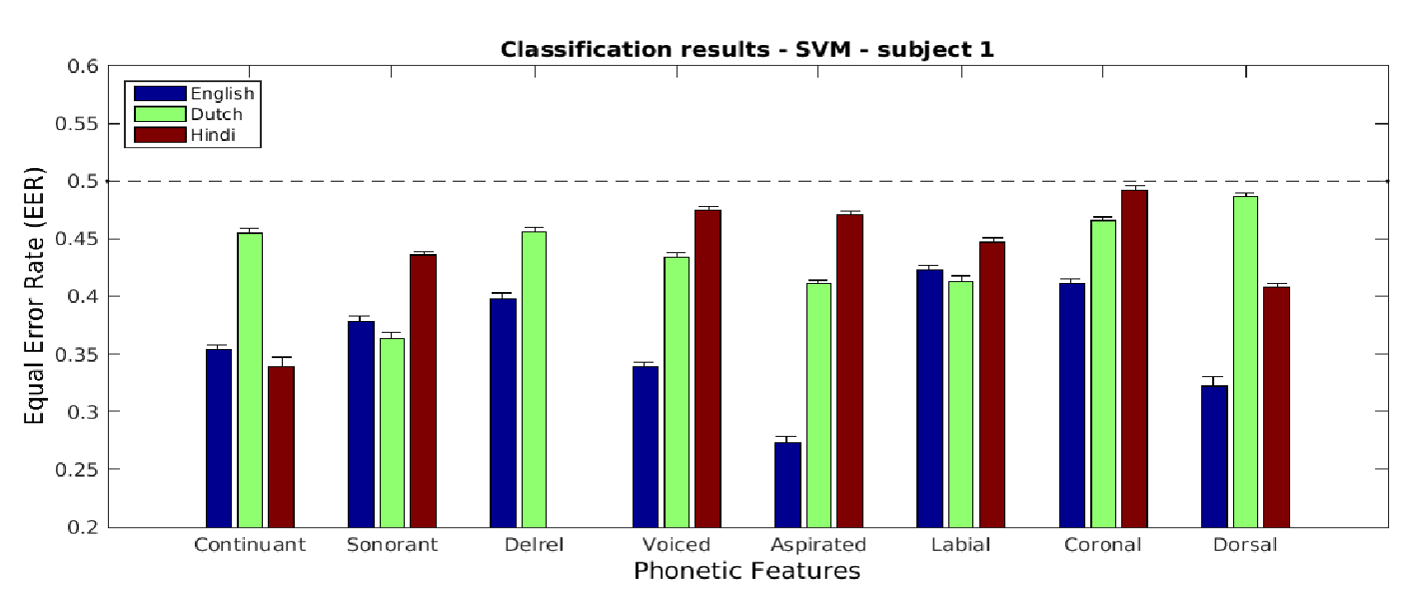
\includegraphics[width=5in]{../figs/diliberto_svmresults.png}}
  \caption{Classifiers were trained to observe EEG signals, and to
    classify the distinctive features of the phoneme being audited.
    Equal error rates are shown for English (the language used in
    training; train and test data did not overlap), Dutch, and Hindi
    (not used in training).}
  \label{fig:eeg_svm_eers}
\end{figure}

Eqs.~\ref{eq:dfdist} defines a log-linear model of $\rho(\psi|\phi)$, the
probability that Dutch phoneme $\phi$ will be perceived as English
phoneme $\psi$.  Denote by $\rho_U(\psi|\phi)$ the model of
Eq.~\ref{eq:dfdist} with uniform weights for all distinctive features
($w_k=\alpha$, a tunable constant).  Denote by $\rho_{EEG}(\psi|\phi)$ the
same model, but with weights $w_k$ derived from EEG measurements
(Eq.~\ref{eq:eegdist}).  Fig.~\ref{fig:eeg_confusions} shows these
two confusion matrices: $\rho_U(\psi|\phi)$ on the left,
$\rho_{EEG}(\psi|\phi)$ on the right.  The figure clearly shows the
difference between these two distributions.  The entropy of the
uniform distribution, $\rho_U(\psi|\phi)$, is too low: when a Dutch
phoneme $\phi$ has a nearest-neighbor $\psi^*(\phi)$ in English, then
few other phonemes are considered to be possible confusions.
$\rho_{EEG}(\psi|\phi)$ has a very different problem: since distinctive
feature classfiers have been trained for only a small set of
distinctive features (in particular, no vowel classifiers were
trained), there are large groups of phonemes whose confusion
probabilities can not be distinguished (giving the figure its
block-diagonal structure).  The faults of both models can be
ameliorated by interpolating them in some way, e.g., by computing the
linear interpolation
$\rho_I(\psi|\phi)=a\rho_U(\psi|\phi)+(1-a)\rho_{EEG}(\psi|\phi)$ for some
constant $0\le a\le 1$.

\begin{figure}
  \centerline{
    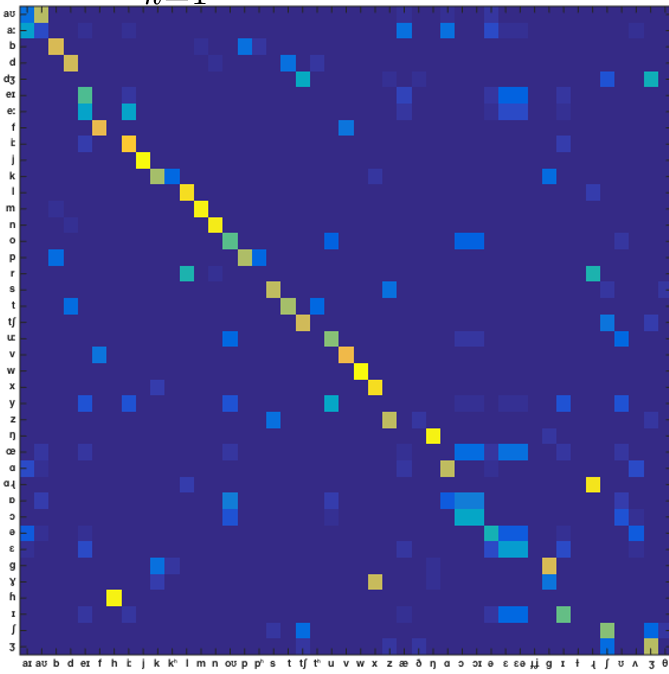
\includegraphics[width=3in]{../figs/mirbagheri_dist_features.png}
    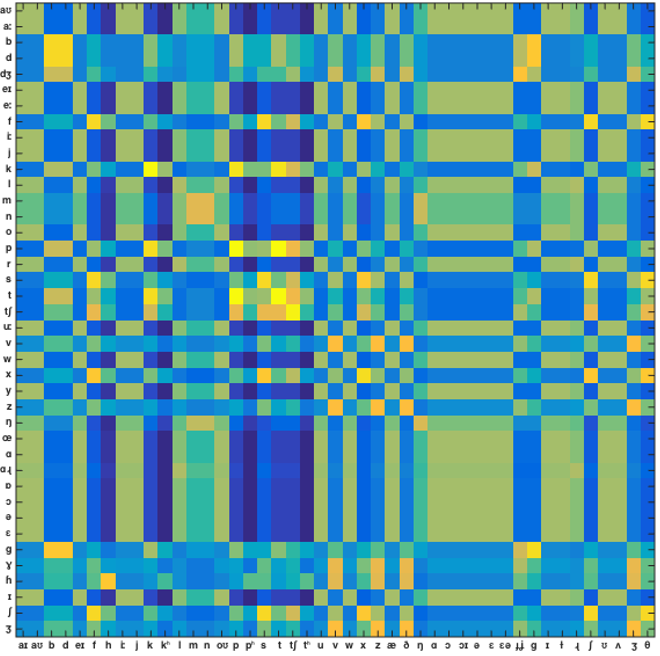
\includegraphics[width=3in]{../figs/mirbagheri_dist_eeg.png}
  }
  \caption{Phoneme confusion probabilities between English phonemes
    (column) and Dutch phonemes (row) using models in which the log
    probability is proportional to distance between the corresponding
    distinctive feature vectors.  Left: all features have the same
    weight.  Right: feature weights equal negative log error rate of
    EEG signal classifiers.}
  \label{fig:eeg_confusions}
\end{figure}
    
